\begin{figure}[!h]
	\centering
    \begin{subfigure}{0.48\textwidth}
    %%\centering
	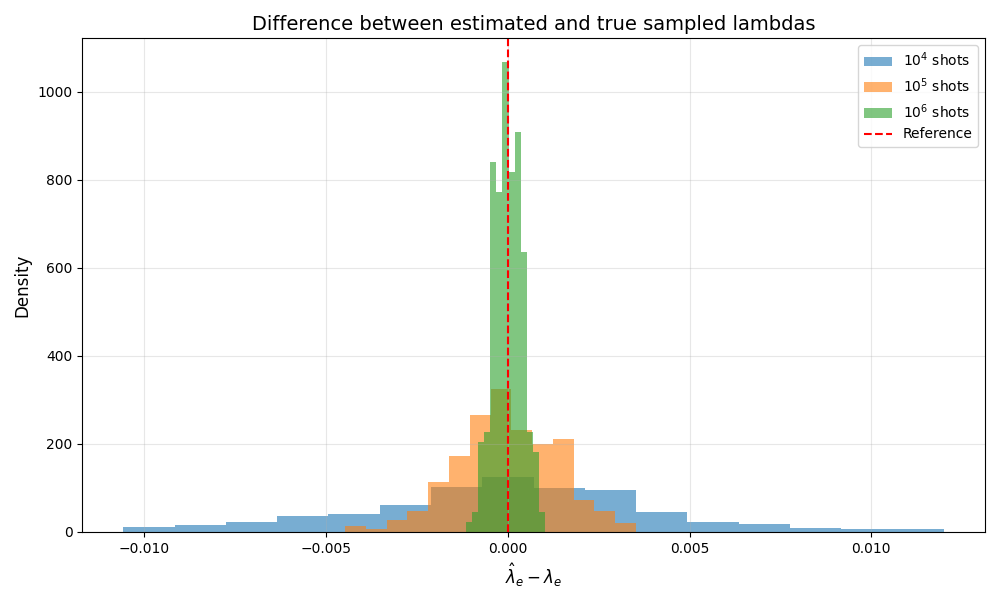
\includegraphics[width=\linewidth]{plot_lambda_diff_by_shots_sd.png}
    %\caption{}
	%\caption{Distribution of the reconstruction differences for the 2D cluster-state with $12 \times 12$ simulation, shown for $10^4$, $10^5$, and $10^6$ shots. The dashed red line indicates zero difference. The distribution becomes increasingly concentrated around zero as the number of shots increases.}
	%\label{fig:lambda_diff_by_shots}
    \end{subfigure}
\hfill
\begin{subfigure}{0.48\textwidth}
	%\centering
	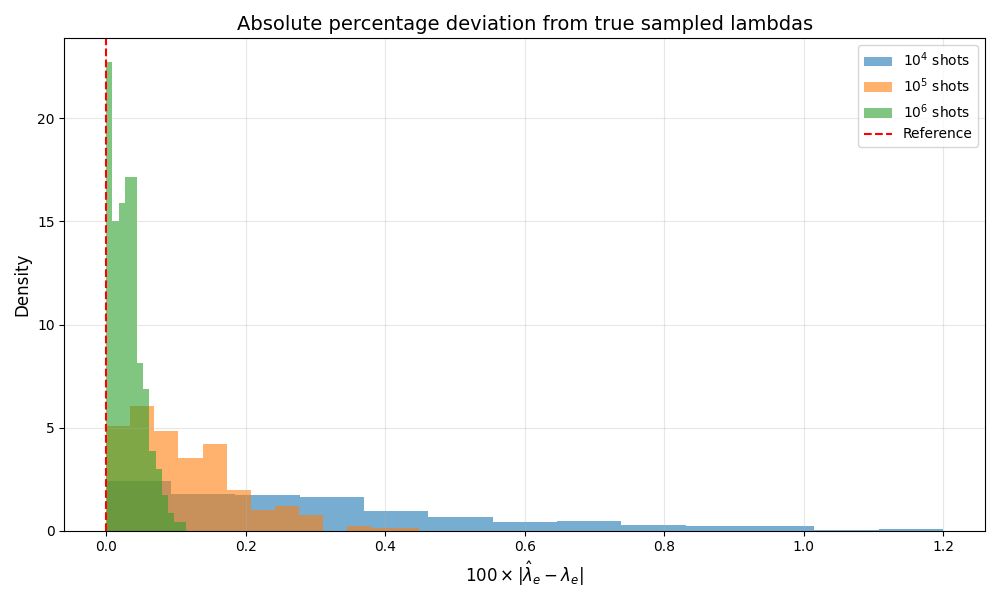
\includegraphics[width=\linewidth]{plot_lambda_diff_abs_by_shots_sd.png}
    %\caption{}
	%\caption{Distribution of the absolute reconstruction deviations for the 2D cluster-state with $12 \times 12$ simulation, shown for $10^4$, $10^5$, and $10^6$ shots. The improved concentration near zero with increasing shot count indicates better reconstruction accuracy.}
	%\label{fig:lambda_abs_diff_by_shots}
\end{subfigure}
%%\vspace{-0.4cm}
\caption{Distribution of the reconstruction differences $\widehat{\lambda}_e-\lambda_e$
(left) and of the absolute deviations $100\times |\widehat{\lambda}_e-\lambda_e|$ (right)
for the $12\times 12$ 2D cluster-state, using $10^4$, $10^5$, and $10^6$ shots, when the
post-$\CZ$ one-qubit depolarizing error probabilities are sampled independently from
$\mathcal{N}(10^{-2},\,2\times 10^{-3})$. The dashed red line marks zero difference. As the
number of shots increases, the signed-error distribution sharpens around zero and the absolute
deviations become more concentrated near zero, indicating improved reconstruction accuracy.}
%\caption{Distribution of the reconstruction differences for the 2D cluster-state with $12 \times 12$ simulation, shown for $10^4$, $10^5$, and $10^6$ shots. The dashed red line indicates zero difference. The distribution becomes increasingly concentrated around zero as the number of shots increases (left). Distribution of the absolute reconstruction deviations for the 2D cluster-state with $12 \times 12$ simulation, shown for $10^4$, $10^5$, and $10^6$ shots. The improved concentration near zero with increasing shot count indicates better reconstruction accuracy (right).}
\label{fig:lambda_diff_by_shots}
\end{figure}
%%\hfill
%%\vspace{-0.8cm}
\begin{figure}[!h]
    \centering
    \begin{subfigure}{0.48\textwidth}
    \centering
	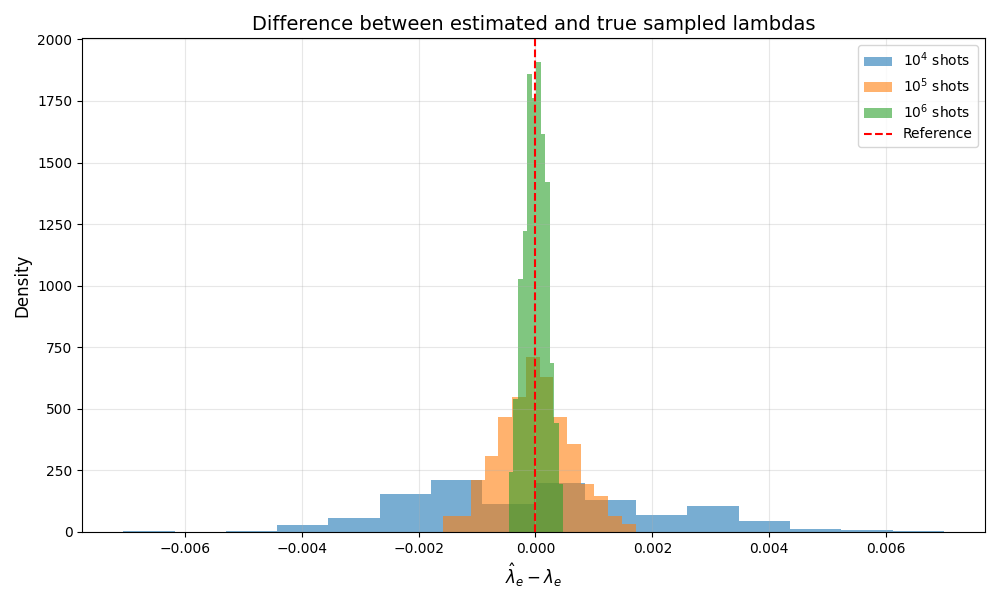
\includegraphics[width=\linewidth]{plot_lambda_diff_by_shots_sd_0002.png}
    %\caption{}
	%\caption{Distribution of the reconstruction differences for the 2D cluster-state with $12 \times 12$ simulation, shown for $10^4$, $10^5$, and $10^6$ shots. The dashed red line indicates zero difference. The distribution becomes increasingly concentrated around zero as the number of shots increases.}
	%\label{fig:lambda_diff_by_shots}
    \end{subfigure}
\hfill
\begin{subfigure}{0.48\textwidth}
	\centering
	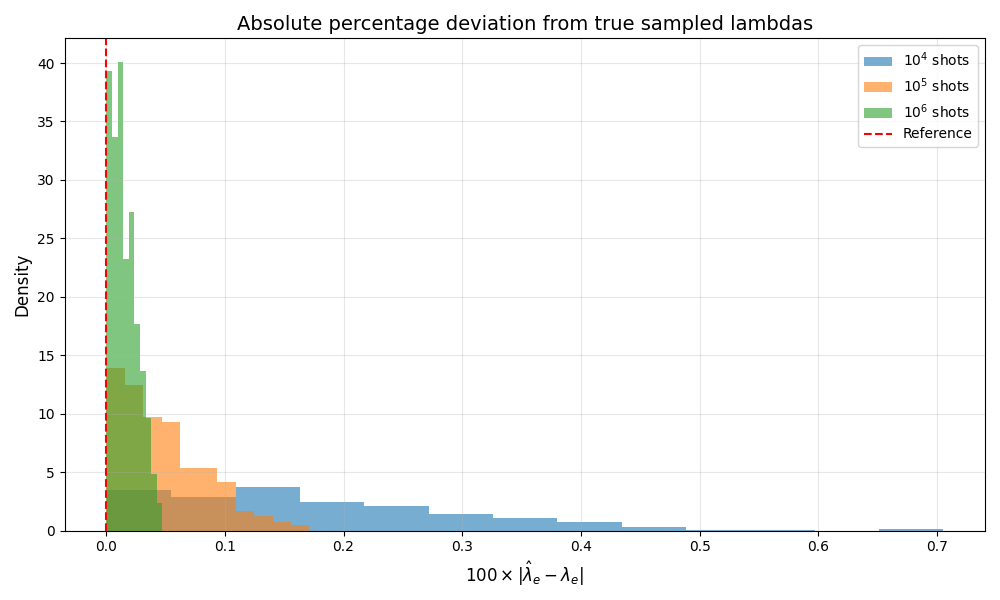
\includegraphics[width=\linewidth]{plot_lambda_diff_abs_by_shots_sd_0002.png}
    %\caption{}
	%\caption{Distribution of the absolute reconstruction deviations for the 2D cluster-state with $12 \times 12$ simulation, shown for $10^4$, $10^5$, and $10^6$ shots. The improved concentration near zero with increasing shot count indicates better reconstruction accuracy.}
	%\label{fig:lambda_abs_diff_by_shots}
\end{subfigure}
%%\vspace{-0.4cm}
\caption{Distribution of the reconstruction differences $\widehat{\lambda}_e-\lambda_e$
(left) and of the absolute deviations $100\times |\widehat{\lambda}_e-\lambda_e|$ (right)
for the $12\times 12$ 2D cluster-state, using $10^4$, $10^5$, and $10^6$ shots, when the
post-$\CZ$ one-qubit depolarizing error probabilities are sampled independently from
$\mathcal{N}(10^{-2},\,2\times 10^{-4})$. The dashed red line marks zero difference. The
reconstruction is centered near zero and becomes progressively more concentrated as the shot
count increases.}
 %   \caption{Distribution of the reconstruction differences for the 2D cluster-state with $12 \times 12$ simulation, shown for $10^4$, $10^5$, and $10^6$ shots. The dashed red line indicates zero difference. The distribution becomes increasingly concentrated around zero as the number of shots increases (left). Distribution of the absolute reconstruction deviations for the 2D cluster-state with $12 \times 12$ simulation, shown for $10^4$, $10^5$, and $10^6$ shots. The improved concentration near zero with increasing shot count indicates better reconstruction accuracy (right).}
    %\label{fig:placeholder}
\end{figure}
%%\hfill
%\vspace{-0.8cm}
    \begin{figure}[!h]
	\centering
    \begin{subfigure}{0.48\textwidth}
    %\centering
	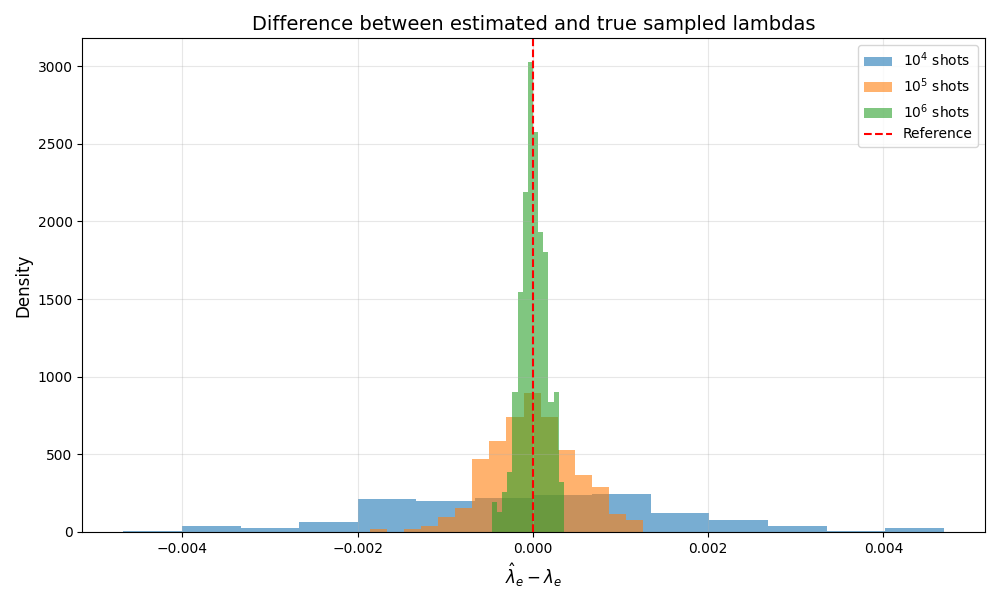
\includegraphics[width=\linewidth]{plot_lambda_diff_by_shots}
    %\caption{}
	%\caption{Distribution of the reconstruction differences for the 2D cluster-state with $12 \times 12$ simulation, shown for $10^4$, $10^5$, and $10^6$ shots. The dashed red line indicates zero difference. The distribution becomes increasingly concentrated around zero as the number of shots increases.}
	%\label{fig:lambda_diff_by_shots}
    \end{subfigure}
\hfill
\begin{subfigure}{0.48\textwidth}
	%\centering
	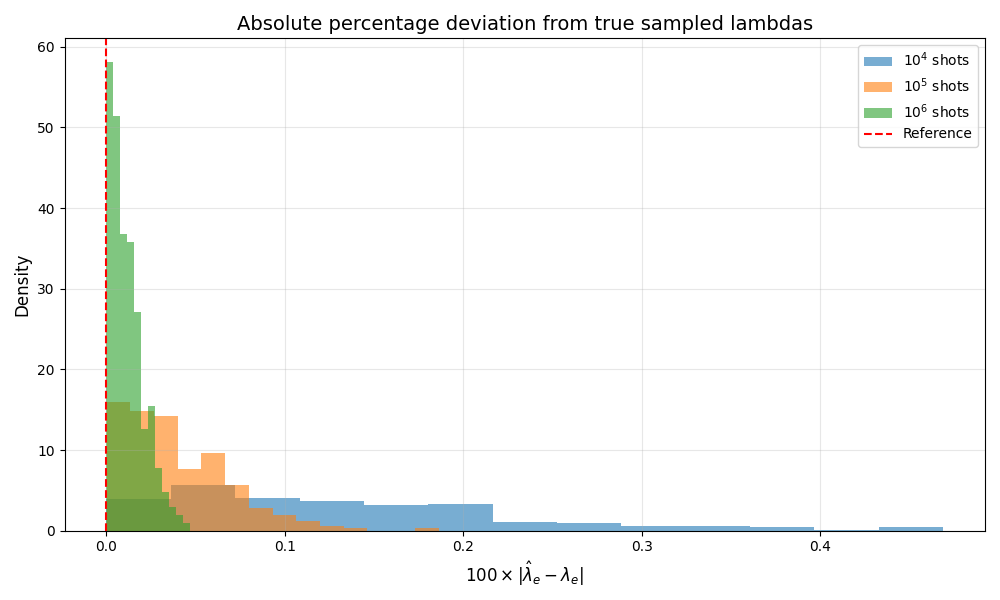
\includegraphics[width=\linewidth]{plot_lambda_diff_abs_by_shots}
    %\caption{}
	%\caption{Distribution of the absolute reconstruction deviations for the 2D cluster-state with $12 \times 12$ simulation, shown for $10^4$, $10^5$, and $10^6$ shots. The improved concentration near zero with increasing shot count indicates better reconstruction accuracy.}
	%\label{fig:lambda_abs_diff_by_shots}
\end{subfigure}
%\vspace{-0.4cm}
\caption{Distribution of the reconstruction differences $\widehat{\lambda}_e-\lambda_e$
(left) and of the absolute deviations $100\times |\widehat{\lambda}_e-\lambda_e|$ (right)
for the $12\times 12$ 2D cluster-state, using $10^4$, $10^5$, and $10^6$ shots, when the
post-$\CZ$ one-qubit depolarizing error probabilities are sampled independently from
$\mathcal{N}(10^{-2},\,2\times 10^{-5})$. The dashed red line marks zero difference. The
signed and absolute reconstruction errors both contract as more samples are collected.}
  %  \caption{Distribution of the reconstruction differences for the 2D cluster-state with $12 \times 12$ simulation, shown for $10^4$, $10^5$, and $10^6$ shots. The dashed red line indicates zero difference. The distribution becomes increasingly concentrated around zero as the number of shots increases (left). Distribution of the absolute reconstruction deviations for the 2D cluster-state with $12 \times 12$ simulation, shown for $10^4$, $10^5$, and $10^6$ shots. The improved concentration near zero with increasing shot count indicates better reconstruction accuracy (right).}
    %\label{fig:placeholder}
\end{figure}
%%\hfill
%\vspace{-0.4cm}
\begin{figure}[!h]
	\centering
    \begin{subfigure}{0.48\textwidth}
    %\centering
	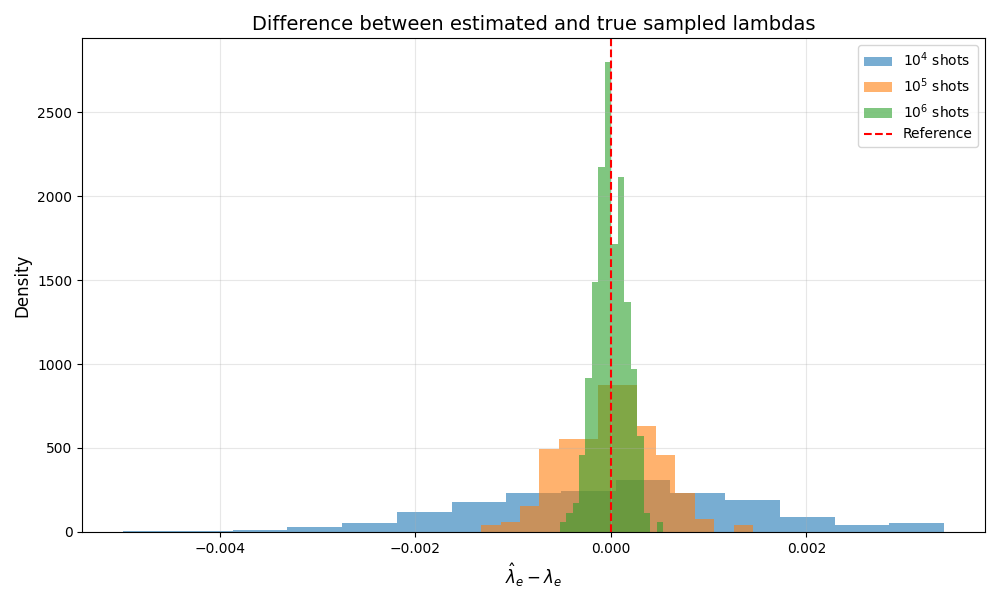
\includegraphics[width=\linewidth]{plot_lambda_diff_by_shots_sd_000002.png}
    %\caption{}
	%\caption{Distribution of the reconstruction differences for the 2D cluster-state with $12 \times 12$ simulation, shown for $10^4$, $10^5$, and $10^6$ shots. The dashed red line indicates zero difference. The distribution becomes increasingly concentrated around zero as the number of shots increases.}
	%\label{fig:lambda_diff_by_shots}
    \end{subfigure}
\hfill
\begin{subfigure}{0.48\textwidth}
	%\centering
	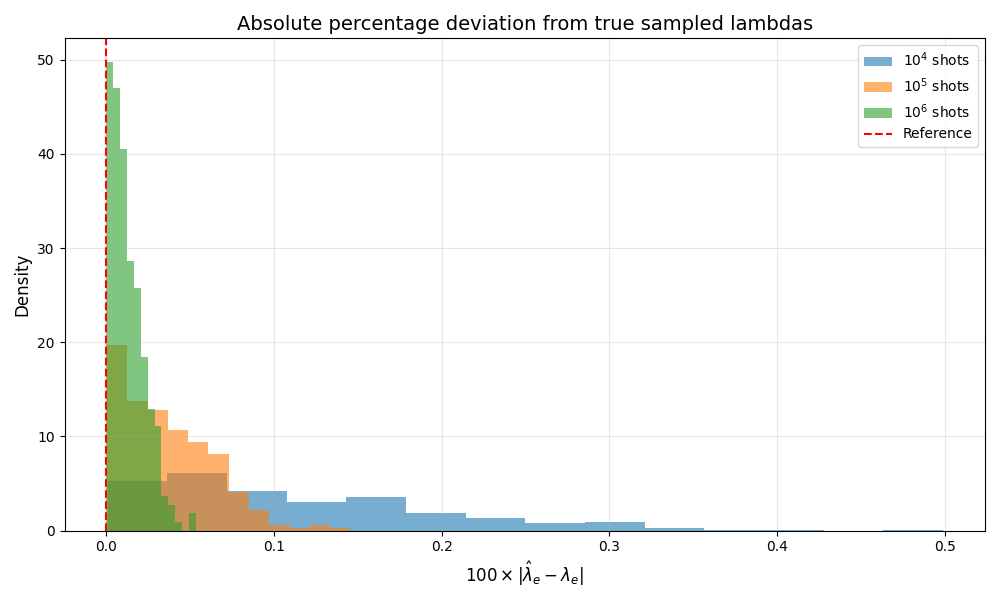
\includegraphics[width=\linewidth]{plot_lambda_diff_abs_by_shots_sd_000002.png}
    %\caption{}
	%\caption{Distribution of the absolute reconstruction deviations for the 2D cluster-state with $12 \times 12$ simulation, shown for $10^4$, $10^5$, and $10^6$ shots. The improved concentration near zero with increasing shot count indicates better reconstruction accuracy.}
	%\label{fig:lambda_abs_diff_by_shots}
\end{subfigure}
%\vspace{-0.4cm}
\caption{Distribution of the reconstruction differences $\widehat{\lambda}_e-\lambda_e$
(left) and of the absolute deviations $100\times |\widehat{\lambda}_e-\lambda_e|$ (right)
for the $12\times 12$ 2D cluster-state, using $10^4$, $10^5$, and $10^6$ shots, when the
post-$\CZ$ one-qubit depolarizing error probabilities are sampled independently from
$\mathcal{N}(10^{-2},\,2\times 10^{-6})$. The dashed red line marks zero difference. The
histograms remain centered near zero, while increasing the number of shots reduces the spread
of the reconstruction error.}
%    \caption{Distribution of the reconstruction differences for the 2D cluster-state with $12 \times 12$ simulation, shown for $10^4$, $10^5$, and $10^6$ shots. The dashed red line indicates zero difference. The distribution becomes increasingly concentrated around zero as the number of shots increases (left). Distribution of the absolute reconstruction deviations for the 2D cluster-state with $12 \times 12$ simulation, shown for $10^4$, $10^5$, and $10^6$ shots. The improved concentration near zero with increasing shot count indicates better reconstruction accuracy (right).}
    %\label{fig:placeholder}
\end{figure}
%%\hfill
%\vspace{-0.4cm}
\begin{figure}[!h]
	\centering
    \begin{subfigure}{0.48\textwidth}
    %\centering
	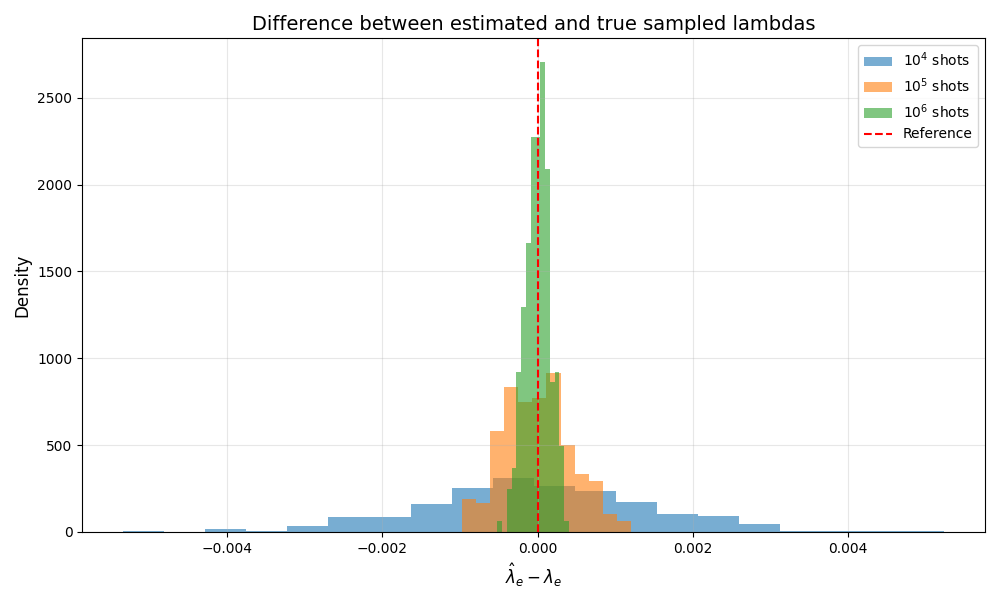
\includegraphics[width=\linewidth]{plot_lambda_diff_by_shots_sd_0000002.png}
    %\caption{}
	%\caption{Distribution of the reconstruction differences for the 2D cluster-state with $12 \times 12$ simulation, shown for $10^4$, $10^5$, and $10^6$ shots. The dashed red line indicates zero difference. The distribution becomes increasingly concentrated around zero as the number of shots increases.}
	%\label{fig:lambda_diff_by_shots}
    \end{subfigure}
\hfill
\begin{subfigure}{0.48\textwidth}
	%\centering
	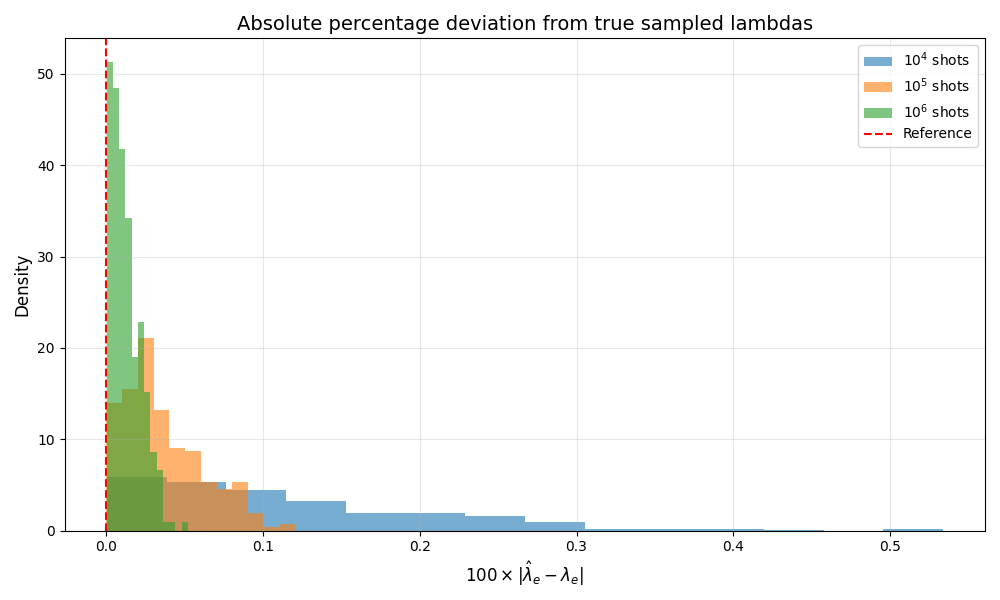
\includegraphics[width=\linewidth]{plot_lambda_diff_abs_by_shots_sd_0000002.png}
    %\caption{}
	%\caption{Distribution of the absolute reconstruction deviations for the 2D cluster-state with $12 \times 12$ simulation, shown for $10^4$, $10^5$, and $10^6$ shots. The improved concentration near zero with increasing shot count indicates better reconstruction accuracy.}
	%\label{fig:lambda_abs_diff_by_shots}
\end{subfigure}
%\vspace{-0.4cm}
\caption{Distribution of the reconstruction differences $\widehat{\lambda}_e-\lambda_e$
(left) and of the absolute deviations $100\times |\widehat{\lambda}_e-\lambda_e|$ (right)
for the $12\times 12$ 2D cluster-state, using $10^4$, $10^5$, and $10^6$ shots, when the
post-$\CZ$ one-qubit depolarizing error probabilities are sampled independently from
$\mathcal{N}(10^{-2},\,2\times 10^{-7})$. The dashed red line marks zero difference. This is
the most concentrated noise ensemble among the five cases, and the reconstruction errors shrink
further as the shot count increases.}
%\caption{Distribution of the reconstruction differences for the 2D cluster-state with $12 \times 12$ simulation, shown for $10^4$, $10^5$, and $10^6$ shots. The dashed red line indicates zero difference. The distribution becomes increasingly concentrated around zero as the number of shots increases (left). Distribution of the absolute reconstruction deviations for the 2D cluster-state with $12 \times 12$ simulation, shown for $10^4$, $10^5$, and $10^6$ shots. The improved concentration near zero with increasing shot count indicates better reconstruction accuracy (right).}
\label{fig:lambda_abs_diff_by_shots}
\end{figure}